
\begin{figure*}[b]
    \centering
    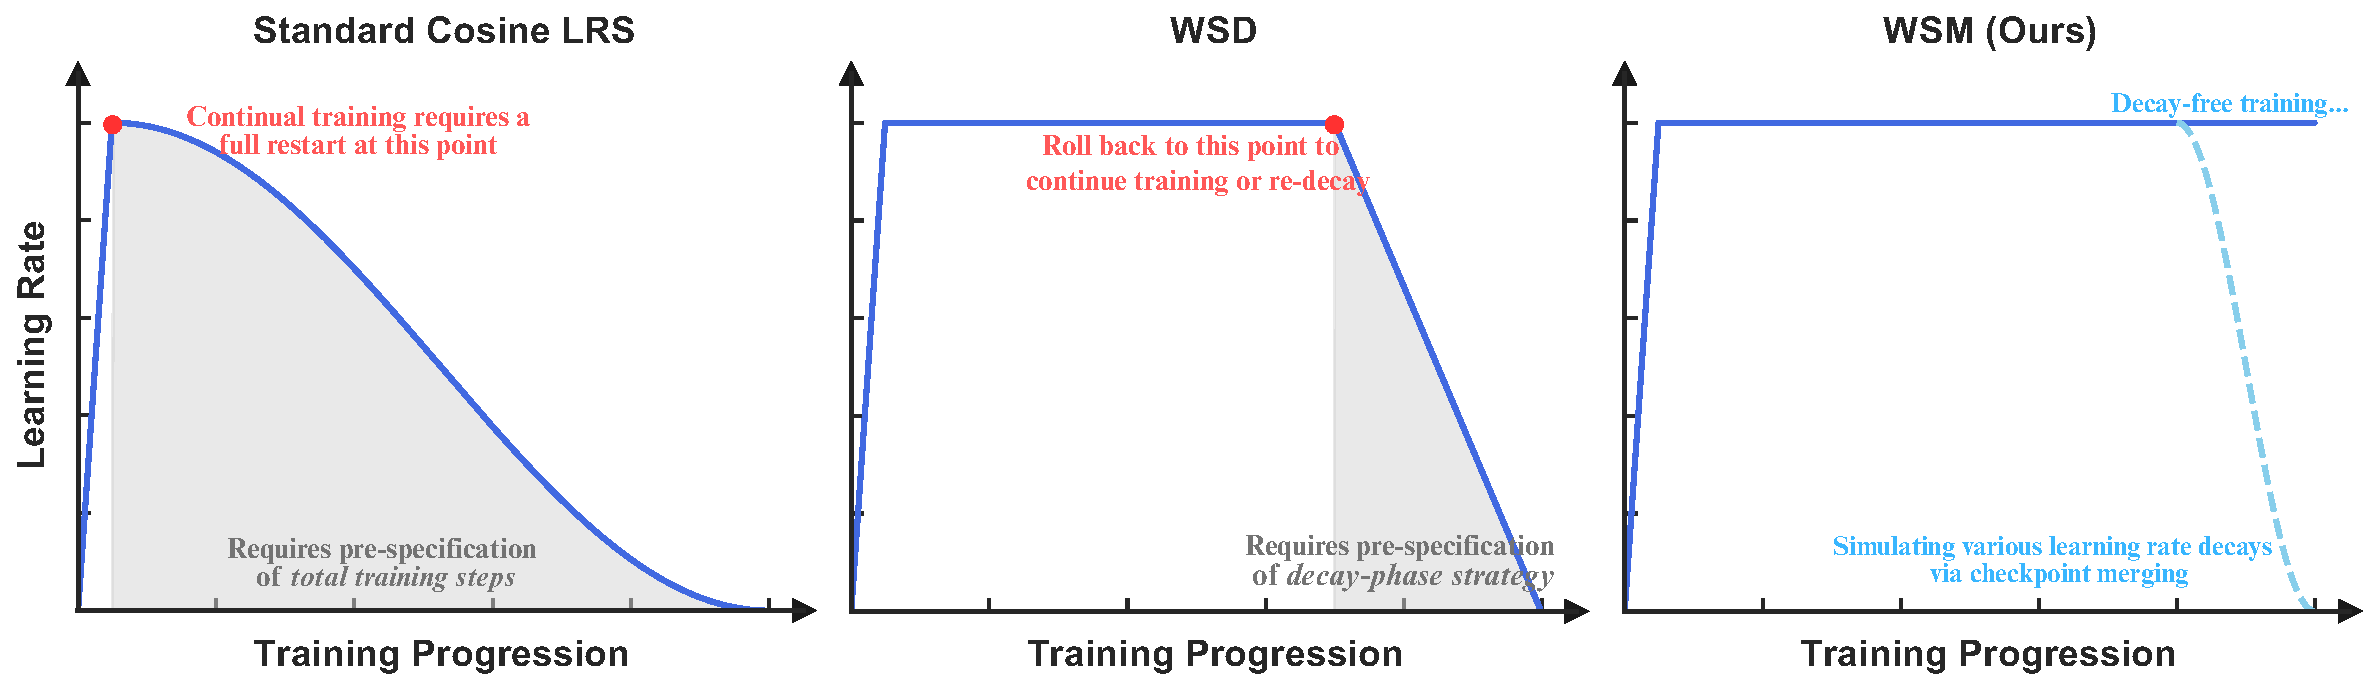
\includegraphics[width=1.\textwidth]{figs/learning_rate_schedules.pdf.pdf}
    \caption{\textbf{Comparison between WSM (Warmup-Stable and Merge) and mainstream learning rate scheduling strategies.}
    By leveraging checkpoint merging, WSM eliminates the learning rate decay phase and maintains a constant learning rate after warmup, enabling a fully autonomous and continuous training process.}
    \label{fig:lrs}
\end{figure*}

\section{Introduction}

In large language model (LLM) pre-training, learning rate (LR) scheduling plays a pivotal role, critically impacting training stability, convergence speed, and final model performance~\citep{Rethinking,Akhilesh}. Conventional LR schedules dynamically adjust the LR based on training progress, with the cosine decay schedule emerging as a widely-adopted approach~\citep{kaplan2020scaling,hoffmann2022training}. This method features an initial warm-up phase followed by cosine-based decay, both constrained by a \emph{predetermined} total training duration. Consequently, any extension of the training process, such as incorporating new data, necessitates a complete restart from the beginning to recalibrate the entire decay curve. 

To address this inflexibility, the Warmup-Stable-Decay (WSD) strategy~\citep{minicpm} inserts a \emph{stable training}  phase with a constant LR between the warmup and decay phases. This schedule provides two key advantages: (1) flexible initiation of the decay phase independent of total step count, and (2) complete decoupling from fixed training durations. The WSD approach has demonstrated significant effectiveness, evidenced by its adoption in several recent LLMs including DeepSeek-V3~\citep{deepseekv3} and  ERNIE 4.5~\citep{ernie2025technicalreport}. %
However, WSD introduces new scheduling requirements: researchers must manually decide when to initiate the decay, how many tokens to allocate for it, and which decay function (e.g., cosine, linear) to employ. Furthermore, if training needs to be extended after the decay has commenced, one must roll back the training to the state preceding the decay phase and re-design the decay strategy. This dependency on a manually configured schedule counteracts the goal of a fully autonomous and continuous training process. 








To minimize scheduling complexity, recent research has investigated alternative approaches that completely eliminate the decay phase from LR schedules~\citep{Aaron2024Road,song2025through,Hanlin2025cbs}. A prominent direction in this field explores weight averaging (a.k.a., model merging) techniques. Empirical results demonstrate that simply maintaining a constant LR combined with standard weight averaging strategies—such as exponentially weighted averaging (EWA)—can achieve performance competitive with WSD-based schedules~\citep{pma}. Building upon this line of research, we make three key extensions: 

(1) We present \emph{Warmup-Stable and Merge (WSM)}, a simple yet general framework for LR scheduling. By formalizing the connection between LR decay and checkpoint merging, we demonstrate that WSM can be instantiated to emulate various decay strategies—including cosine decay, linear decay and inverse square root (1-sqrt) decay. Our framework provides a principled approach to convert any LR decay method into a theoretically approximate model averaging implementation. This contrasts with prior work~\citep{Aaron2024Road,song2025through,pma}, which has largely focused on analysis of specific averaging strategies and their optimization properties. Notably, our framework is optimizer-agnostic, enabling seamless integration with various optimization algorithms (e.g., SGD, Adam) without requiring modifications on the underlying training pipeline.

(2) Through extensive experiments, we systematically investigate key factors in instantiating this framework, including merge methods, merge frequency, duration, granularity, and the compatibility of merging and decay strategies. Our findings reveal that merge duration—the training period covered by the merged checkpoints—emerges as the most critical factor influencing model performance, with significantly greater impact than both the checkpoint interval and the number of merged models.

(3) The proposed decay-free LR schedule delivers substantial performance gains. Extensive empirical evaluation shows consistent improvements across multiple benchmarks: +3.5\% on MATH, +2.9\% on HumanEval, and +5.5\% on MMLU-Pro—a significant advance over the WSD method, while prior work often only matches WSD's performance. Moreover, these benefits naturally extend to the post-training stage, demonstrating our method's potential for sustained improvements in long-term model refinement.














The proposed WSM framework presents a promising direction for developing effective decay-free LR schedules. Our results demonstrate consistent performance advantages across both pre-training and fine-tuning stages. Notably, WSM enables the implementation of sophisticated decay-like methods through a simple and stable optimization approach, combining the benefits of strategic scheduling with robust training dynamics.












